% !TEX root = ../main.tex

\chapter{相关工作}

\section{手势的定义与身体姿态的参数化表示}

\subsection{手势的定义与范围}

在人类交流中,手势(gesture)是与语音同时出现的重要非语言信号,它承担语义补充、情感表达与互动调节等多重功能。McNeill(1992)\cite{mcneill_1992_hand}提出,手势并非语言的附属物,而是语言思维的外化形式,是语音与思维之间的中介过程。Kendon(2004)\cite{kendon_2004_gesture}进一步指出,手势涵盖从手部动作、头部运动到上身姿态的广义身体行为,构成“可见的发话(visible utterance)”。在此框架下,手势与语言并非分离系统,而是同源于共同的认知与表达机制。

\paragraph{手部手势的分类}
McNeill将随语音出现的手部手势划分为四个基本类型,这一分类构成了当代手势研究与生成建模的重要语义基础:

\begin{enumerate}
  \item \textbf{Iconic gestures(形象性手势)}:以具象方式描绘事物的外形、空间路径或动作特征,例如用手势勾勒一个圆形或表示“上升”的轨迹。此类手势与语言内容直接对应,表达具体语义。
  \item \textbf{Metaphoric gestures(隐喻性手势)}:表达抽象概念或思维结构的手势,如用手的展开表示“扩展话题”或“阐述概念”。它们并不描绘实体,而以隐喻形式具象化抽象语义。
  \item \textbf{Deictic gestures(指示性手势)}:指向空间中的对象、人物或方向,常用于对话焦点的指明与注意引导,如“指向你”“指向那边”等。
  \item \textbf{Beat gestures(拍击型手势)}:与语音重音、韵律或节奏结构同步的节奏性动作,不承载具体语义,但用于强调语音节奏与结构边界。它们体现了语言与动作在时间组织上的耦合。
\end{enumerate}

这四类手势既体现了语言—动作系统的语义层次,也为计算模型提供了不同的生成目标维度。在自然交流中,它们往往混合出现,但在建模与生成任务中,通常根据可观测特征与任务目标加以区分。

\paragraph{头部手势的分类}
与手部动作类似,头部姿态在语音交流中同样承担多种沟通功能。
Wagner、Malisz 与 Kopp(2014)\cite{gesture_and_speech_in_interaction}将头部运动视为语音—动作协同系统的一部分,
并指出头部点动、摆动等刚体运动在时间结构上常与手势及语音节奏保持同步。
基于其语用与韵律功能,可将常见头部手势归纳为以下几类:
\begin{itemize}
  \item \textbf{韵律型(Prosodic head gestures)}:与语音重音、节奏同步的周期性点动或摆动,
        强调语音节奏与句法边界,是“beat 手势”的头部对应形式;
  \item \textbf{语义型(Semantic or attitudinal head gestures)}:用于表达肯定、否定、疑问或强调等态度性语义,
        常与发话语义或情绪一致;
  \item \textbf{指向型(Deictic head gestures)}:通过转头、注视方向指示互动对象或话题焦点;
  \item \textbf{预测型(Predictive cues)}:在语音重读之前出现的微小点头或抬头动作,
        作为即将发声或重读的提前信号\cite{busso2007rigidheadmotion}。
\end{itemize}
这些类型与手部手势的四分类在功能上相互补充,共同构成人类多模态语音交互的节奏与语义层结构。

\subsection{身体姿态的参数化表示}
在计算机动画与动作捕捉领域,身体姿态通常由骨架结构(skeleton hierarchy)和关节旋转参数(joint rotations)共同定义。骨架结构描述了人体各关节的拓扑关系及层级依赖;而每个姿态帧(pose frame)由一组关节旋转参数所确定,这些参数定义了相对于父节点的旋转变换。在不同的系统与任务中,骨架结构的具体形式往往有所差异,这种差异直接影响姿态数据的表示与学习方式。

在不同的系统与任务中,骨架结构可以遵循各自的标准,因此,不同的数据集、3D 模型或神经网络往往基于自身定义的关节层级与命名体系进行训练与标注。例如,AMASS 数据集采用 SMPL 拓扑结构,BEAT 数据集使用简化上半身骨架,而部分生成模型仅选取躯干与手臂关节以满足实时计算需求。近年来,自动骨骼绑定与骨架归一化技术的发展在一定程度上消除了不同拓扑结构之间的差异,使得模型和数据间的姿态映射更加一致。

在确定骨架结构之后,具体的姿态状态可通过多种旋转参数进行描述。常见的旋转参数表示方法包括:

\begin{enumerate}
\item 欧拉角(Euler Angles):通过三个顺序旋转角表示姿态,直观但存在“万向节锁(gimbal lock)”问题;
\item 四元数(Quaternion):以四维单位向量表示旋转,避免奇异性,但在神经网络训练中不易约束;
\item Axis-Angle:以旋转轴与旋转角度组合的形式表示,参数紧凑但角度不连续;
\item Rot6d\cite{rot6d}:将旋转矩阵前两列展开为六维向量,通过归一化保持正交性,连续性与可学习性兼具。
\end{enumerate}

在计算机图形与实时渲染中,通常采用四元数或旋转矩阵进行骨骼变换与插值,以保证数值稳定性和计算效率。
然而,在深度学习任务中,这些表示在高维空间中存在不连续性或约束难度。近年来的研究表明\cite{rot6d},Rot6d 表示在动作生成与姿态预测任务中具有更好的连续性与可学习性,可显著提升模型的收敛特性与泛化性能。
因此,本文在姿态生成模型中统一使用 Rot6d 表示每个关节的旋转状态,以确保训练阶段的平滑收敛与推理阶段的稳定性。

不同的手势生成方法在旋转参数的选取上各不相同,相关实例见表~\ref{fig:rotation_comparison}。

\begin{table}[htbp]
\centering
\caption{不同旋转表示方式的空间连续性与使用示例}
\label{fig:rotation_comparison}
\begin{tabular}{@{}lcccc@{}}
\toprule
\textbf{表示方式} & \textbf{维度} & \textbf{连续性} & \textbf{典型应用场景} & \textbf{使用示例} \\ \midrule
欧拉角 & 3 & 存在万向节锁 & 图形学、传统动画 & CaMN\cite{beatcamn} \\
四元数 & 4 & 连续 & 实时渲染、骨骼动画 & — \\
Axis-Angle & 4 & 角度部分不连续 & 动作预测、生成任务 & DiffSHEG\cite{diffsheg} \\
Rot6d & 6 & 连续 & 深度学习生成模型 & EMAGE\cite{emage} \\ \bottomrule
\end{tabular}
\end{table}

\section{面部表情的定义与参数化表示}

面部表情是非语言交流的重要组成部分,与语音、手势共同传递情感和态度信息。与身体动作不同,面部表情主要由皮肤形变和局部运动构成,无法通过骨骼旋转直接建模,因此需要专门的参数化表示方式。

目前常见的面部状态描述方法主要有两类:

\paragraph{BlendShape 权重模型}
BlendShape 将面部表情表示为一组线性可加的形变基(morph targets),每个基形由一个实值权重控制,最终表情由各基形按权重叠加得到。其方法论与 FACS 中的 Action Units (AU) 一致:复杂表情可以被分解为若干可组合的基本动作单元。

BlendShape 模型具有标准化、可实时驱动、与动画系统兼容等优点,因此被广泛应用于 ARKit \cite{ARKitDocumentation} 等实时捕捉系统,并被主流渲染引擎采用。

\begin{figure}[h!t]
\centering
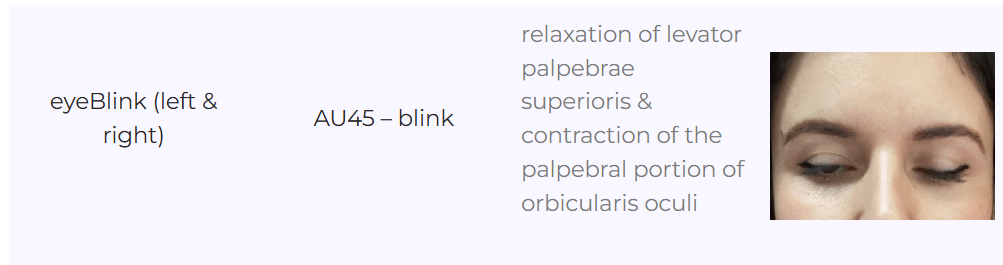
\includegraphics[width=0.95\linewidth]{figures/Fig_AUSample.png}
\caption{示例图来自~\cite{ozel_arkit_facs_cheatsheet},展示 FACS AU45(blink)对应的 ARKit 中的两种 BlendShape 基形:\texttt{eyeBlinkLeft}(闭左眼)与 \texttt{eyeBlinkRight}(闭右眼)。}
\label{fig:au_sample}
\end{figure}

图~\ref{fig:bs_eyeblink} 展示了 \texttt{eyeBlinkLeft}、\texttt{eyeBlinkRight} 基形在权重 $w\!\in\![0,1]$ 下的线性插值效果(从张眼到闭眼)。这使得 BlendShape 向量既便于作为可学习输入,又可直接映射到渲染引擎的驱动接口。

\begin{figure}[h!t]
\centering
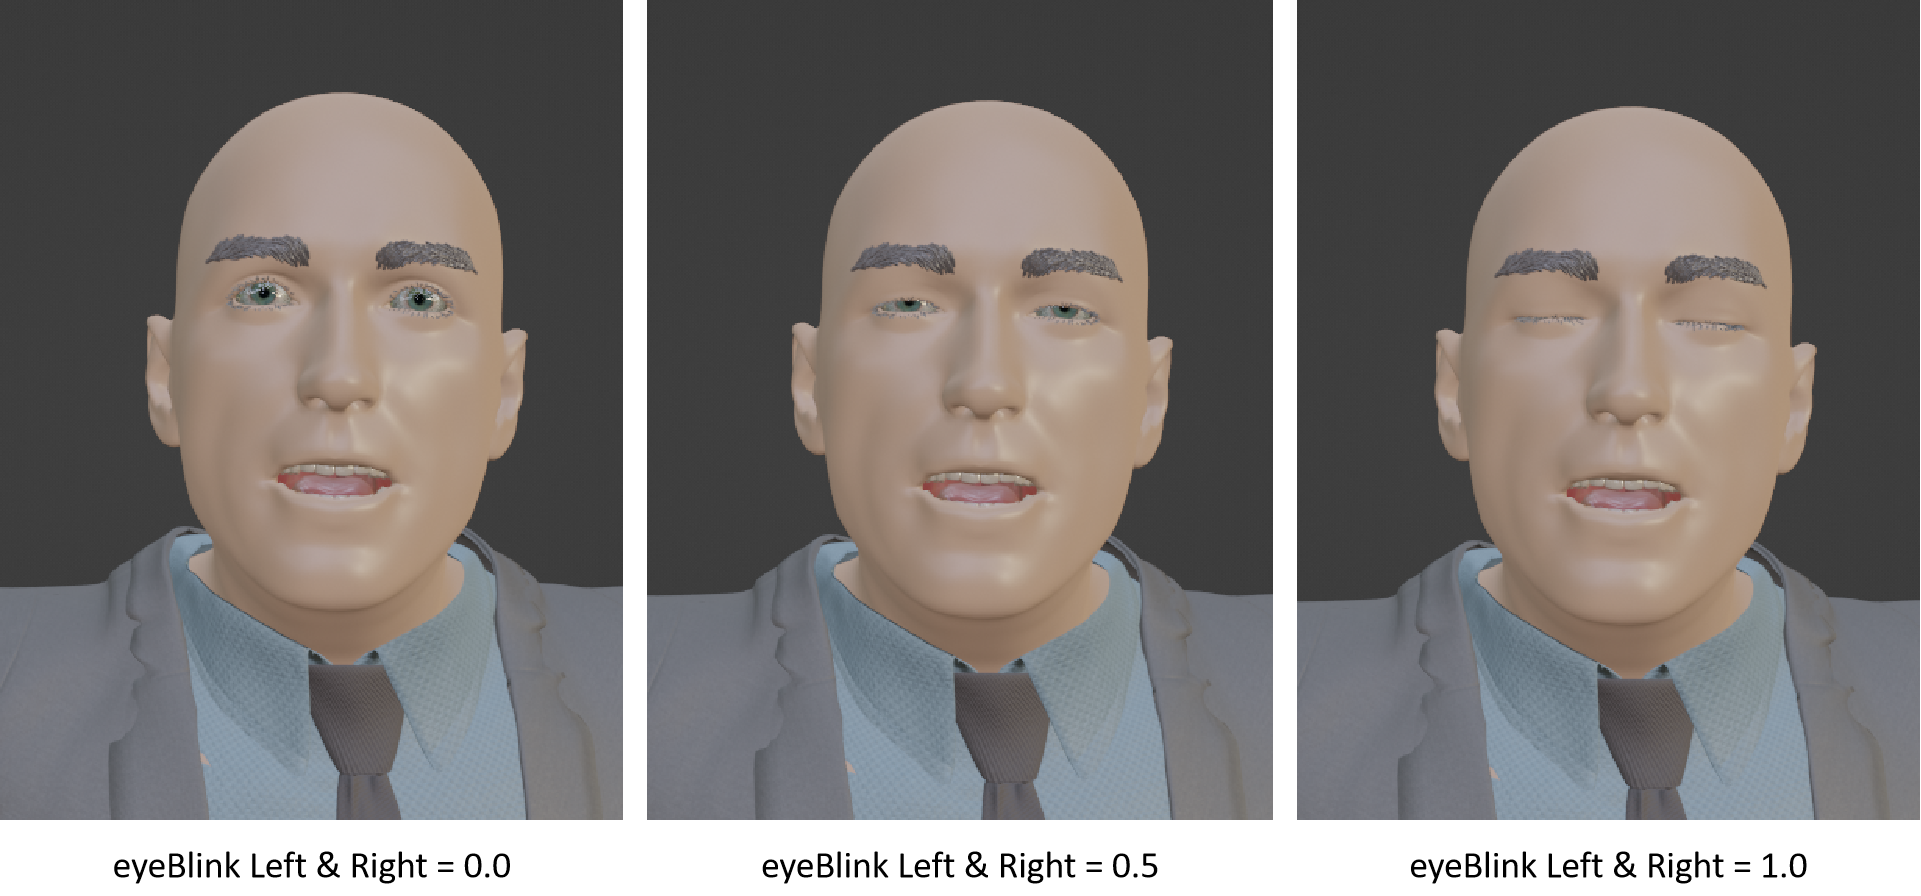
\includegraphics[width=0.95\linewidth]{figures/Fig_blendshapeEyeBlink.png}
\caption{BlendShape 线性插值效果示例:\texttt{eyeBlink} 从 $w{=}0$(左)到 $w{=}1$(右)的连续变化,中图为中间值。BS 权重可直接用于实时渲染驱动。}
\label{fig:bs_eyeblink}
\end{figure}

在具有相同网格结构的角色模型之间,BlendShape 基形集合可以直接复用,但在拓扑不同的模型间则需重新定义。

\paragraph{关键点坐标模型(Landmark-based Representation)}
关键点模型通过检测面部若干语义特征点(2D 或 3D 坐标)来描述几何结构变化。典型实现包括 MediaPipe Face Mesh \cite{mediapipefacemesh} 与 OpenFace 系列。

与基于网格形变的 BlendShape 不同,关键点模型并不依附于任何具体网格拓扑,而是在几何空间中以语义一致的特征点集合形式定义面部结构。这种表示方式并不描述模型的形变,而是对“人脸几何”的抽象建模,因此常用于表情识别、头部姿态估计等分析任务,而较少用于驱动渲染。

在多模态学习与特征分析中,BlendShape 表示具有较高的统一性和可量化性,适合以固定维度向量作为模型输入,并易于应用于不同虚拟角色的动画驱动。因此,本文在系统设计中采用与 ARKit 兼容的 BlendShape 参数作为面部模态输入特征。

\begin{figure}[h!t]
\centering
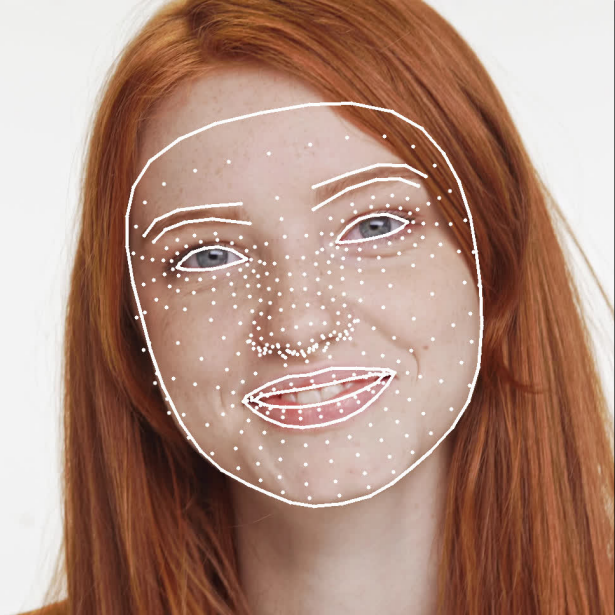
\includegraphics[width=0.4\linewidth]{figures/Fig_MediaPipeLandmark.png}
\caption{MediaPipe Face Mesh 关键点结构示意图,截取自 \cite{mediapipefacemesh}。}
\label{fig_mediapipe_landmark}
\end{figure}

\section{国内外研究现状}

\subsection{手势生成的研究目标}

\subsubsection{研究目标类型的差异}

语音驱动的手势生成研究在总体目标上虽一致——即让虚拟角色的动作与语音内容、节奏协调一致——但在使用场景与系统角色上存在显著差异。

现有研究大体可分为两类:

\paragraph{为AI的虚拟形象生成手势}

这一类研究的目标是让AI驱动的文本对话系统的虚拟形象具备手势表现力。

模型可以一次性生成下一句语音或文本,因此可以访问完整的未来信息,包括整句音频、文本和语义上下文。

典型方法通过编码完整句子的节奏与语义,预测整段动作轨迹,以最大化动作与语义的一致性和整体流畅性。

这类方法适合AI驱动的系统或离线生成的应用场景,如合成视频。

\paragraph{为用户的虚拟人生成实时手势}
本文所聚焦的目标类型属于第二类。

在用户实时说话的过程中,系统需根据当前语音流(以及可选的面部与头部模态)即时生成同步手势。

此任务具有严格的实时性约束与因果性限制:模型在每一时刻只能使用当前及过去的信息,而不能访问未来语音或文本内容。

因此,常见的整句式规划或滑动预测方法不再适用。

该任务更接近实时交互系统,而非内容生成系统。

\subsubsection{任务约束与可利用条件的差异}

这两类研究目标在可利用的信息条件和评价重心上存在本质区别:

\begin{table}[h]
\centering
\caption{两类手势生成任务在约束与可利用条件上的对比}
\label{tab:task_constraint_comparison}
\begin{tabular}{@{}p{3cm}p{5.5cm}p{5.5cm}@{}}
\toprule
\textbf{对比维度} & \textbf{AI 虚拟形象生成} & \textbf{用户虚拟人实时生成} \\ 
\midrule
输入信息 & 完整句级语音或文本(可使用未来信息) & 实时语音流,仅使用过去与当前帧 \\ 
输出目标 & 整句手势序列(离线生成) & 连续流式手势(逐帧生成) \\ 
时间约束 & 不必要实时 & 帧级实时性($<$50\,ms 推理延迟) \\ 
评价重点 & 整体语义一致性与美学自然度 & 瞬时同步性、动作平滑与交互稳定性 \\ 
应用场景 & 离线动画、内容合成、AI虚拟直播 & 实时虚拟人、视频会议、用户虚拟直播 \\ 
\midrule
语音模态 & 作为输入或由文本生成(TTS 输出) & 作为实时输入特征(语音流) \\ 
手部手势 & 生成目标(输出) & 生成目标(输出) \\ 
面部表情 & 通常为生成目标(输出) & 可通过设备实时采集,作为输入辅助推理 \\ 
头部姿态 & 通常为生成目标(输出) & 可实时采集并作为输入特征,用于同步推理 \\ 
\bottomrule
\end{tabular}
\end{table}

前者可以在生成阶段规划动作节奏与语义对应,而后者需在无未来信息的条件下维持自然与同步,
并保证输出连续、平滑且无突跳,从而对模型结构、输入模态与延迟控制提出更高要求。

\subsubsection{评估方法}

语音驱动手势生成研究的评价体系通常涵盖生成质量、时序匹配与表达多样性等多个维度。
研究者既关注生成动作的自然性与视觉流畅度,也重视其与语音信号在节奏和语义层面的对应关系。
近年来,随着实时生成和多模态扩展任务的发展,相关评估方法也逐渐体系化,可概括为以下几类:

\begin{enumerate}
    \item \textbf{自然性(Naturalness)} —— 衡量生成动作在运动平滑性、速度变化及能量分布上的合理性,常采用 FGD(Fréchet Gesture Distance)\cite{ginosar2019speech2gesture}、
          运动速度统计、或主观“自然度”评分等指标。
    \item \textbf{同步性(Synchronization)} —— 评估手势在时间上与语音重音或韵律事件的对齐程度,
          常用 BA(Beat Alignment)\cite{kucherenko2021predictability}、DTW(Dynamic Time Warping)等方法,
          以及基于重读检测的主观同步性评价。
    \item \textbf{多样性(Diversity)} —— 衡量模型在不同语音输入下生成的动作变化程度,
          通常以轨迹分布的方差、速度曲线差异或 L1DIV 等指标度量,
          以防止模型陷入单一模式或过度平滑。
    \item \textbf{语义相关性(Semantic Relevance)} —— 反映生成动作与语义关键词或情绪类别的一致性,
          可通过 SRGR(Semantic Relevance to Gesture Ratio)\cite{beatcamn} 等指标或人工标注语义标签对齐评估。
    \item \textbf{实时性与稳定性(Latency \& Robustness)} —— 在面向交互系统的研究中,
          还需评估帧级推理延迟与输出平滑性,以确保动作流连续且系统响应及时。
\end{enumerate}

总体而言,现有评价体系既包含客观的运动学与统计指标,也结合主观感知评分,
在不同任务目标下可形成“自然性—同步性—多样性—相关性”的综合评估框架。

\subsection{手势生成的演变}

近年来,语音驱动手势生成经历了从规则设计到数据驱动模型、再到多模态扩展与实时生成的持续演变。
这一过程不仅体现了算法架构的更新,也反映了研究目标与应用场景的变化:
从基于语言规则的行为映射,到学习语音—动作关系的深度生成模型,再到面向交互的多模态实时系统。

\subsubsection{规则驱动阶段}

早期的手势生成系统主要依赖语言学规则与专家知识构建 \cite{behavior_expression_animation_toolkit,robot_behavior_toolkit,gesture_generation_by_imitation,gesture_and_speech_in_interaction}。
这类方法通过语义分类或韵律规则将语音片段映射为预定义的手势模板(如指示、肯定、节奏性动作),并以有限的动作库组合出手势序列。
典型代表如 BEAT toolkit 与 Robot Behavior Toolkit,它们可在虚拟代理或机器人中实现基于语音的同步动作。
然而,手势词典与语法规则的人工设计成本较高,难以覆盖自然语音中的多样变化,导致生成结果缺乏自然性与个体差异。

\subsubsection{数据驱动阶段}

随着大规模语音与动作配对数据的出现,研究者开始采用统计学习和深度神经网络模型学习语音—手势映射关系。
在此阶段,语音通常作为唯一输入模态,模型通过 LSTM、GRU 或 MLP 等结构预测连续手势序列。
典型代表如 CaMN 模型 \cite{beatcamn},其基于 BEAT 数据集 \cite{beatcamn} 训练级联网络,将 LSTM、全连接网络与 GAN 结构相结合,实现从语音到动作的端到端预测。

然而,该类模型多使用欧拉角或离散旋转参数作为手势表示,生成结果容易出现抖动与不连续。
后续工作引入更平滑的表示方式,如 Rot6d \cite{rot6d,emage,AMUSE2024} 或 Axis-Angle \cite{diffsheg},显著提升了动作流畅性。
与此同时,为解决语音与手势间的多对多映射问题,研究者引入了 VQ-VAE \cite{emage,zhang2024SemanticGesticulator} 与扩散模型 \cite{tamingDiffgesture,diffsheg,diffstylegesture,DiffTED2024,diffusion-self-supervised2023},
在保持自然性的同时提升了生成多样性与表现力。

尽管这些方法在客观指标与视觉效果上均优于传统模型,但它们普遍假设可访问完整语音或文本上下文,
属于“整句式(non-streaming)”生成,推理延迟较高,不适用于实时应用。
即便是推理效率较高的模型(如 CaMN、DiffSHEG),也因上下文缓冲机制而引入明显延迟。

\subsubsection{多模态扩展阶段}

为进一步提升动作表现力与语音理解能力,部分研究引入视觉模态或语言语义特征。
例如,CaMN \cite{beatcamn} 在语音输入的基础上融合面部捕捉信息以增强表现;
EMAGE \cite{emage} 与 DiffSHEG \cite{diffsheg} 同时生成手势与面部动作;
DiffTED \cite{DiffTED2024} 更进一步,实现了端到端的视频合成,使虚拟角色的语音、面部与肢体同步生成。

这些多模态生成方法在提升虚拟智能体的自然感与沉浸感方面表现优异,但其任务假设仍基于整句输入,因此主要用于AI 虚拟形象生成或离线内容创作场景,而非实时用户交互。

\subsection{当代生成研究的策略趋势}
尽管 McNeill 的分类提供了语义层面的参考,但实际的手势生成任务常针对可观测与可学习的特征进行抽象。近年的研究在数据建模层面主要呈现三种策略:

\begin{enumerate}
  \item \textbf{简化标签法(Simplified labeling)}:为降低多部位、多语义类别手势的标注与分类难度,
    研究者通常将所有身体层动作(包括手部与头部)统一划分为
    “节奏型(beat-like)”与“语义型(semantic-like)”两大类,
    而不再严格遵循 McNeill 针对手部动作的四类划分。
    这种方式在语音—动作对齐任务中更具可操作性,
    特别适用于以韵律为核心驱动的生成模型。
    由于节奏型(beat-like)手势与头部动作均与语音韵律的时间结构高度耦合,
    现有研究往往采用此简化策略,即不对数据集进行显式语义类别标注,
    而仅通过语音—动作对齐学习可观测的节奏模式。
    这种策略可视为“弱标签化(weakly-labeled)”的实现形式,能够避免语义标注成本,并在实时生成任务中取得稳定的同步效果。
  \item \textbf{语义增强方向(Semantic-aware generation)}:部分工作尝试通过语义或文本特征扩展生成范围,以覆盖 \emph{iconic} 或 \emph{metaphoric} 手势。例如 Yoon 等(2020)\cite{yoon2020speechgesturebert} 将语音与文本嵌入结合;Alexanderson 等(2023)\cite{alexanderson2023diffgesture}引入上下文风格控制,实现了语义相关的动作变化。
  \item \textbf{混合式生成策略(Hybrid generation)}:以数据驱动的节奏型(beat-like)底流确保全时连续与韵律对齐,在检测到关键语义事件时,通过规则/检索/模板短片段进行语义强化,并在边界处通过速度与加速度匹配实现无缝过渡。该思路得到近期综述与语义检索式系统的支持\cite{zhang2024SemanticGesticulator},同时 BEAT 数据集提供的语义相关性标签可直接作为触发信号\cite{beatcamn},便于工程化落地。与纯数据驱动的扩散式手势生成\cite{alexanderson2023diffgesture,tamingDiffgesture}以及实时多模态生成\cite{diffsheg}相比,混合式能够在不牺牲节奏自然度的前提下,增强语义显著时刻的表达力。
\end{enumerate}

\section{实时生成的理论基础与可行性分析}
从生成可行性的角度,现有研究普遍认为 \emph{beat} 手势可在无语义理解的条件下由语音韵律直接驱动生成。
大量语音驱动手势研究证实,仅凭语音的能量、时长与音高变化即可合成自然的节奏性上肢动作\cite{ginosar2019speech2gesture,alexanderson2020stylegestures,kucherenko2021movingfastslow}。
这些研究所生成的动作在时间结构上与语音重音同步,体现了语音与手势共享的时间规划机制。

相比之下,\emph{iconic}(形象性)、\emph{metaphoric}(隐喻性)与 \emph{deictic}(指向性)手势均依赖语义或指向关系,需要对话语境或文本语义输入,
难以在严格实时的因果条件下生成。Kucherenko 等\cite{kucherenko2021predictability} 的可预测性分析进一步验证了这一点:
他们发现手势的语义类别和空间指向性在语音特征中几乎不可预测,即便结合文本特征,预测性能也相当有限,
而节奏阶段(phase)相关特征在音频中则具有显著更高的可预测性。
这表明,在缺乏未来语义与全局上下文的实时场景中,仅凭语音模态,模型只能稳定生成节奏层面的动作。

然而,本文的研究在此基础上进一步引入了\emph{头部姿态模态}作为补充输入信号。
与手部动作相比,头部姿态能直接反映注意、指向和互动焦点等空间要素。
因此,虽然 \emph{deictic} 手势在语音和文本模态中难以预测,
但结合头部姿态输入后,模型可以部分恢复空间指向性信息,
在实时约束下生成具有方向感与互动特征的动作成为可能。
这一点构成了本文模型设计的重要理论依据。

\paragraph{头部姿态模态的建模意义}
头部姿态模态不仅与语音韵律在时序上高度耦合,
还能提供语义与情感层面的补充信号。
其不同类型的头部手势——包括韵律型、语义/态度型、指向型与预测型——
在建模上分别发挥以下作用:
\begin{enumerate}
  \item \textbf{韵律同步:}头部动作与语音重音、句法节奏具有高时间一致性,
        其速度与幅度变化可作为语音能量、时长与重读的外显指标,
        有助于模型捕捉语音节奏结构并增强手势的时间同步性;
  \item \textbf{情绪反馈:}头部的肯定、否定或强调动作提供即时的情感线索,
        在语音语义模糊时帮助模型区分发话倾向与语气;
  \item \textbf{指向与注意:}转头与注视方向反映说话者的注意焦点,
        在时间上为手势触发提供“方向性约束”,
        可提升空间一致性与互动感;
  \item \textbf{预测信号:}微小的预点头或抬头动作往往早于声学重读出现,
        为模型提供时间上的“前瞻信号”,
        以弥补因果条件下缺乏未来语义信息的不足。
\end{enumerate}
从工程角度看,头部姿态输入既能在节奏层面补充韵律一致性,
又能在空间层面提升对话的自然交互感,
因此在实时语音驱动任务中成为极具价值的输入模态。

\paragraph{头部模态补充语音驱动的空间指向性预测}
如前所述,Kucherenko 等\cite{kucherenko2021predictability} 的研究表明,
手势的空间指向性在语音与文本模态中可预测性均较低,
这意味着传统纯语音驱动系统难以生成具有明确空间方向的动作。
然而,头部姿态模态天然携带了空间线索:
其转头与注视变化反映了注意目标与话题焦点,
而预测型点头可提前暗示节奏或发音峰值。
因此,在实时生成模型中,
引入头部模态不仅增强了韵律一致性,
更为生成具方向感的\emph{deictic}类手势提供了信息基础。

尽管如此,模型仍存在边界:
头部模态信号受设备噪声与说话风格差异影响,
难以完全替代语义理解或文本上下文。
因此,本文模型在设计上以 \emph{beat-like} 手势为基石,
保留对 \emph{deictic} 手势的有限触发能力,
而不追求生成 \emph{iconic} 与 \emph{metaphoric} 手势。
这种策略在保证实时性与稳定性的同时,
兼顾空间表达与自然度,为多模态实时生成提供了理论与实践的平衡点。

\section{本文的工作与创新点}

本文研究的目标是设计一种能够在实时条件下运行的语音驱动手势生成模型,使用户无需动作捕捉设备或特定硬件,仅通过语音输入即可驱动虚拟人的上肢与头部动作。与以往主要面向离线生成或 AI 虚拟形象生成的研究不同,本文关注的任务场景是“用户实时交互”,因此系统必须在严格因果的条件下运行,即只能利用当前与过去的输入帧信息,无法依赖未来语音或文本内容进行整体规划。

现有的高精度手势生成模型在离线场景中表现优异,特别是基于扩散模型或 VQ-VAE 的方法 \cite{tamingDiffgesture, diffsheg, emage, DiffTED2024}, 能够生成自然、连贯且语义相关的手势序列。然而,这些模型通常需要整句语音或文本作为输入,推理过程依赖未来信息以分析语义结构与节奏特征,  
因此难以直接应用于实时交互系统。在无未来信息约束下,模型必须在信息不完整的情况下进行预测,这会显著影响动作生成的自然性与语义一致性。

为缓解上述问题,本文提出利用用户的面部表情与头部姿态作为辅助输入模态,为手势生成过程提供额外的非语言信号。面部表情能反映说话者的情绪与语气变化,在语义模糊的情况下有助于生成更具情感表达的动作;头部姿态则能反映注意方向与交互焦点,在语音节奏变化时为手势生成提供时序上的参考。  
通过将这两种模态与语音信号联合输入模型,系统能够在实时条件下获得更多上下文线索,从而在保持低延迟的同时提升手势生成的自然度与一致性。

本文以 CaMN 模型 \cite{beatcamn} 为基础进行扩展。CaMN 原为离线级联结构,输入包括语音与面部捕捉特征,输出包含手部与头部姿态。本文首先将其输入机制改写为逐帧输入流形式,并引入新的头部特征分析模块,将头部姿态信号作为独立通道输入至级联网络的末端层,以强化模型的时序响应能力。  
在这一结构下,系统可在实时语音流输入条件下逐帧生成动作输出,实现语音、面部与头部信号的联合驱动。

实验结果表明,本文提出的模型在实时性与动作自然性之间取得良好平衡。在典型的桌面端环境下,单帧推理时间约为1毫秒之内,能够满足实时交互需求;同时在 FGD、BA 与主观评测中表现出与离线模型相近的手势自然度与同步性。由此,本文的方法证明了在严格因果条件下,通过多模态输入融合可以有效提升实时手势生成的表现力与稳定性。

\section{本章小结}
本章综述了语音驱动手势生成领域的相关研究现状与发展脉络。  
首先,对手势的概念与在计算机中的参数化表示进行了阐述,说明了手势与面部表情、头部姿态在虚拟人交互中的角色与差异。  
随后,从研究目标的角度分析了不同任务设定之间的区别,指出现有大多数工作聚焦于为 AI 虚拟形象生成整句级动作,而缺乏面向用户实时交互的研究。  
在此基础上,回顾了手势生成方法从规则驱动到数据驱动、从单模态到多模态的演变过程,  
总结了现有模型虽在生成质量上取得显著进展,但在实时性与因果性方面仍存在局限。

最后,结合本文的研究目标,提出了面向实时交互的语音驱动手势生成方案。

